\section{Learnings from the winning solutions} \label{sec:winning-solutions}

More than 2500 participants took part in the CRAG competition. Four teams won top-three positions across three tasks, and seven additional teams scored high points for individual question types (see Table \ref{tab:winning-teams}). 

\begin{table}[htbp]
\centering
\caption{CRAG competition winning teams and team placements. For each task we awarded top-3 teams for overall scores, and top-1 team for each question type.}
\begin{tabular}{l|lll}
\toprule
\bf Team name & \bf Task 1 placement & \bf Task 2 placement & \bf Task 3 placement \\
\midrule
db3 \cite{db3} & \bf 1st place& \bf 1st place& \bf 1st place\\
\arrayrulecolor[gray]{0.8}  % 0.7 is medium grey (1 is white, 0 is black)
\hline
APEX \cite{apex} & & \bf 2nd place& \bf 2nd place\\
\hline
md\_dh \cite{mddh} & \bf 2nd place& \bf 3rd place & \makecell[tl]{\\Set\\Aggregation\\Post-processing} \\
\hline
vslyu-team \cite{vslyu} & & & \bf 3rd place \\
\hline
ElectricSheep \cite{electricsheep} & \bf 3rd place & \makecell[tl]{Simple with condition\\Set\\Aggregation\\Multi-hop\\Post-processing}& \\
\hline
dRAGonRAnGers \cite{dragonrangers} & \makecell[tl]{Comparison\\ Post-processing}& Comparison& Comparison\\
\hline
ETSLab & False premise& & Multi-hop\\
\hline
dummy model \cite{dummy_model} & \makecell[tl]{Simple with condition\\Set\\Aggregation} & & \\
\hline
bumblebee7 \cite{bumblebee7} & Multi-hop& & \\
\hline
Future \cite{future} & & False premise & \\
\hline
StarTeam \cite{starteam}& & & Simple with condition\\
\hline
Riviera4 \cite{riviera4} & & & False premise\\
\arrayrulecolor{black}
\bottomrule
\end{tabular}
\label{tab:winning-teams}
\end{table}

Most winning solutions adapt a general RAG system design that comprises two main stages (see Figure \ref{fig:architecture}): (1) Knowledge Retrieval components that retrieve and process relevant information from web or knowledge graphs, and (2) an Augmented Generation component that leverages an LLM to incorporate retrieved information and provide an answer to the question. 

No team trained the overall pipeline in an end-to-end fashion. Instead, each component is optimized separately, where sub-systems are tailored to the specific tasks or question types. The teams leverage both off-the-shelf solutions (e.g., Beautifulsoup for HTML parsing, BGE encoders for ranking) and customized solutions (e.g., fine-tuned LLM to reduce hallucination). In the following we deep dive to learnings from each component.

\begin{figure}[th]
  \centering
  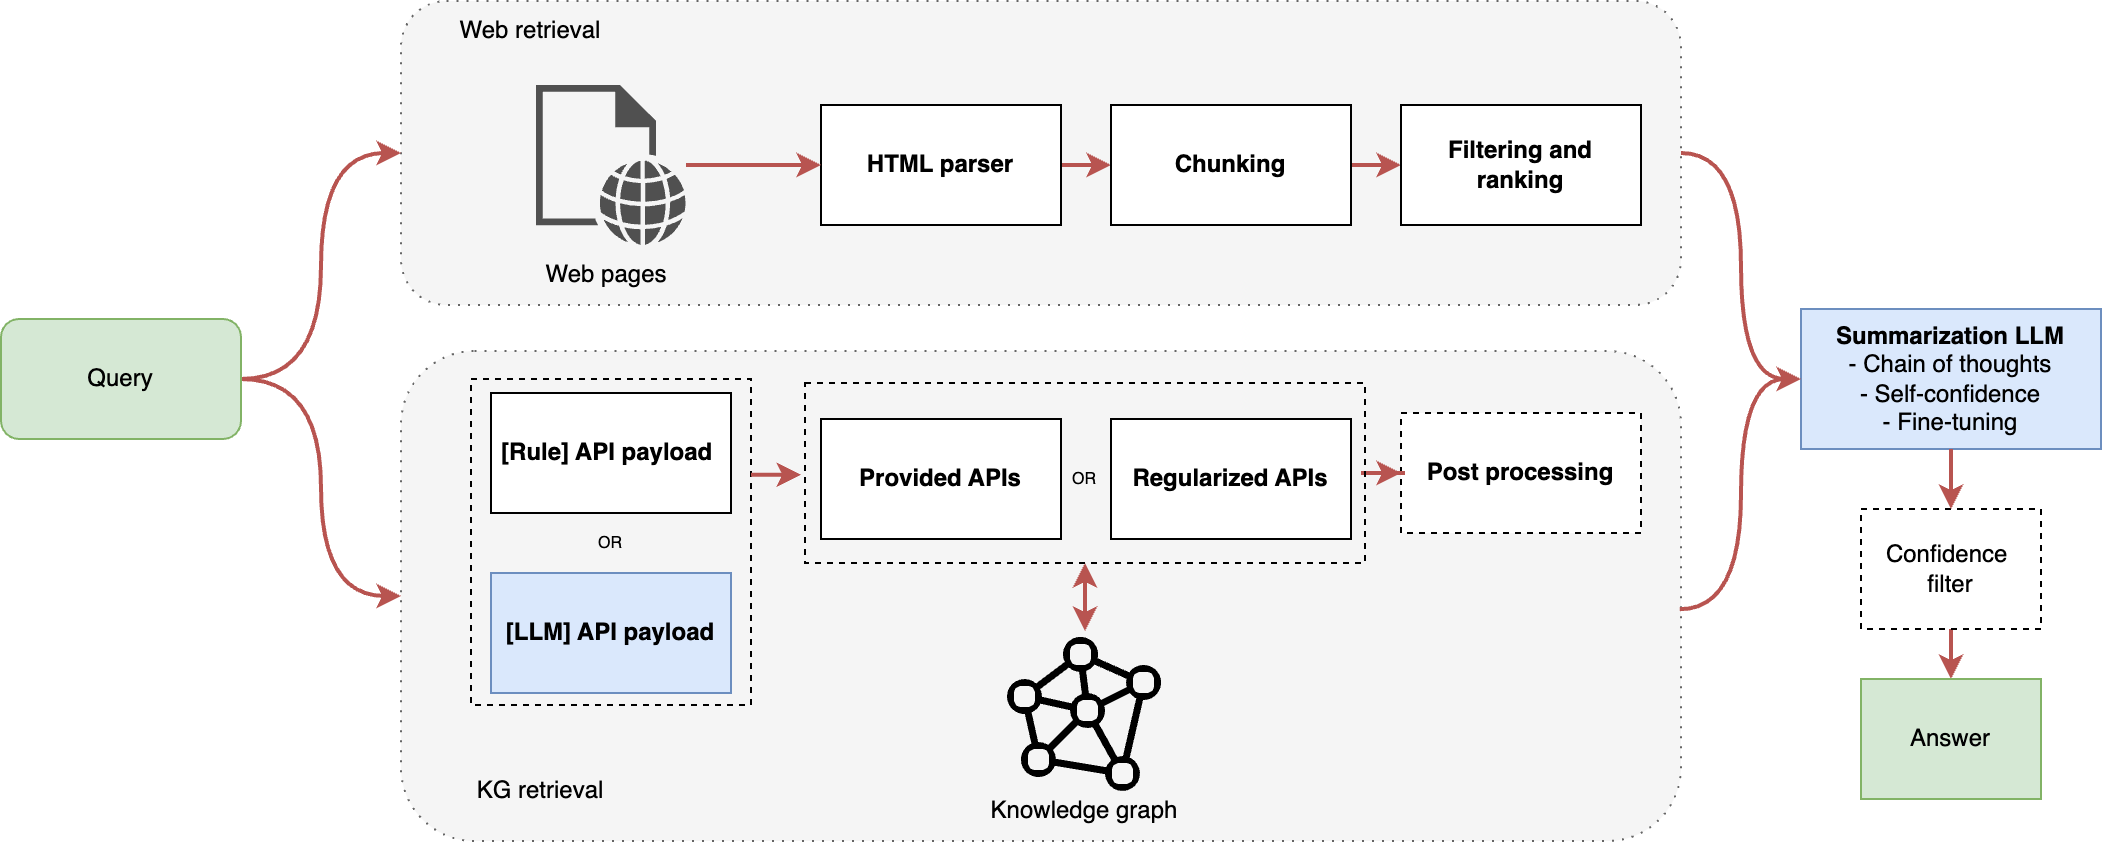
\includegraphics[width=16cm]{submissions/Xiao2024/figs/crag-architecture.drawio.png}
  \caption{Conceptual overall architecture from winning solutions.}
  \label{fig:architecture}
\end{figure}

\subsection{Knowledge Retrieval from Web}
Given a query, this component retrieves supporting material from the web repository (task 1, 2 and 3). An ideal retrieval system finds relevant knowledge efficiently (high recall) without including too many noises (high precision). There are several key challenges: 1) raw HTML contains inconsistent structures, making it challenging to extract clean text; 2) long web pages exceed LLM's input length constraints; 3) webpages often contain contents that are irrelevant to the question that dilute signals and potentially lead to hallucinations from summarizations.

To address these challenges, most winning solutions follow a workflow consisting of four steps to obtain clean relevant information from webpages: HTML parsing, content chunking, relevance scoring, and re-ranking. The teams heavily utilize off-the-shelf libraries as building blocks as listed in Table \ref{tab:tools-web} below.
\begin{table}[htbp]
\centering
\caption{Off-the-shelf libraries the winning solutions leveraged for web retrieval.}
\begin{tabular}{ll}
\toprule
\bf Component & \bf Libraries \\
\midrule
HTML Parsing & BeautifulSoup \cite{richardson2007beautiful}, Trafilatura \cite{barbaresi2021trafilatura} \\
Chunking & CharacterTextSplitter \cite{mavroudis2024langchain} , ParentDocumentRetriever \cite{mavroudis2024langchain}\\
Relevance scoring & bge-base \cite{bge_embedding}, ms-marco-miniLM \cite{ms-marco} , sentence-t5 \cite{ni2021sentence}, BM25 \cite{robertson2009probabilistic}\\
Re-ranking & bge-reranker \cite{chen2024bge}\\
\bottomrule
\end{tabular}
\label{tab:tools-web}
\end{table}

The teams leveraged a variety of \underline{chunking} strategies to partition web content into smaller segments. Beyond the basic token-level chunking method, three solutions stand out in ensuring related contexts are preserved in the same chunk, allowing the summarization model to access coherent information:
\begin{enumerate}
    \item Db3’s \cite{db3} solution maintains a parent-child chunk relationship using the ParentDocumentRetriever library. Once they identify smaller children chunks that are relevant to the question, they include their associated parent chunks in the pipeline.
    \item Md\_dh’s \cite{mddh} solution traverses the tree structure of HTML to identify chunks at node level, minimizing segmentation of texts under a common tag such as header, table, sections.
    \item ElectricSheep’s \cite{electricsheep} solution first identifies questions in web pages by matching sentences that start with ``5W1H'' key words (i.e. "Who", "What", "Where", "When", "Why" and "How") and end with a question mark, and then ensures subsequent texts are grouped together with the questions.
\end{enumerate}

For \underline{relevance scoring} and \underline{re-ranking}, the winning solutions mainly rely on off-the-shelf sparse (e.g. BM25) and dense (e.g. bge-base) retrieval models and re-ranker models (e.g. bge-reranker) without customized fine-tuning. Ablation study (md\_dh \cite{mddh}) shows that dense retrieval via cross-encoders has a slight edge over sparse retrieval in terms of accuracy. 

\subsection{Knowledge Retrieval from KG} \label{sec: kg}
CRAG provides various domain specific APIs to access underlying KG data (task 2,3). The main tasks for efficient retrieval from KG are three folds: 1) identifying the appropriate API(s), 2) generating correct API parameters, and 3) processing API results to find relevant information. 

The winning solutions for KG retrieval fall into three broad categories.
\begin{enumerate}
    \item \underline{Build each retrieval step separately}. Using APEX’s \cite{apex} solution as an example, this approach invokes the following steps. It first leverages an LLM to identify named entities, followed by entity linking via string matches or BM25 fuzzy matches. Then it identifies an appropriate API and its parameters via domain-specific rules and calls the API. Afterwards, it filters the API results based on the date of the query. Finally it converts the filtered results to markdown format and sent to the final generation model. 
    
    This approach provides explicit control and insights of each step at the cost of integration complexity.
    \item \underline{Generate e2e API call directly}. A few teams (db3 \cite{db3}, md\_dh \cite{mddh}, ElectricSheep \cite{electricsheep} etc.) prompt an LLM to directly generate API payload, where fine-tuned LLMs with API specific data further improve the calling accuracy.
    \item \underline{Regularized API}. Another innovative solution came from team db3 \cite{db3}. Instead of building a retrieval system around the original APIs provided by CRAG, the authors develop a new set of \underline{“regularized” APIs} that enhances the expressiveness of the original APIs. More specifically, the solution built API wrappers to encapsulate filtering conditions (e.g.``year” == “2012”) and aggregation logics (e.g. maximum, average). The following is an example comparing the original API and the regularized API.

\begin{equation}
    get\_movie(movie\_name) \rightarrow get\_movie(movie\_name, condition)[key\_name]
\end{equation}
where “condition” is from a set of predefined rules, and “key\_name” are indices to search in the results. The expressive regularized APIs allow the team to obtain concise information via a single API call generated by LLM.
\end{enumerate}

\subsection{LLM Augmented Generation}
LLM Augmented Generation incorporates upstream retrieved knowledge to generate a final answer. All winning solutions put significant efforts in reducing hallucination in this step, partially because hallucination is penalized more severely than a missing (e.g. ``I don’t know") answer in the CRAG scoring criteria. 

The main strategies that the winning solutions adapt to reduce hallucinations are a combination of chain-of-thought prompting, explicit confidence estimation, supervised fine-tuning, and manual rules.

\begin{enumerate}
    \item \underline{Chain-of-thought}. Teams (e.g., ElectricSheep \cite{electricsheep}, APEX \cite{apex}) show that prompting the LLM to articulate intermediate thinking steps improve answering accuracy for complex questions and significantly reduce hallucination. For instance, ElectricSheep \cite{electricsheep} prompts the model to first identify if a question has false premise, then whether the question can be answered by each retrieved evidence, before generating the final answer. 
    \item \underline{Explicit confidence inference}. Another approach is to estimate LLM answer’s confidence, then only retain the answer at high confidence, and answer “I don’t know” otherwise. Winning solutions either prompt the LLM directly to self produce a confidence level, or sample several answering paths and approximate the confidence as the answer consistency. Both methods are effective in their respective pipeline, but the self-consistency approach demands more computational resources.  
    \item \underline{Supervised fine-tuning}. Several teams (e.g., db3 \cite{db3}, md\_dh \cite{mddh}, dRAGonRAnGers \cite{dragonrangers}) fine-tune an Llama-3-8b model specifically targeting reducing hallucinations. The teams generated training labels by first running the pipeline with a non-fine-tuned LLM generation model, then prompts a separate LLM to automatically identify questions that are not answerable by retrieved knowledge passages and labeled “I don’t know” for fine-tuning. The resulting fine-tuned model answers “I don’t know” more frequently on questions that it tends to hallucinate originally. 
    \item \underline{Manual rules}. Since dynamic questions are much more difficult to answer correctly than static questions. Some teams opt to avoid answering dynamic questions all together to prevent getting penalized with hallucinated answers.
\end{enumerate}

\subsection{Observations by Question Categories}
 CRAG categorizes questions along four dimensions: Topic domain (Finance, Sports, Music, Movie, Open), Dynamism (Real-time, Fast-changing, Slow-changing, Static), Popularity (Web, Head, Torso, Tail) and Question Type (Simple, Simple with condition, Set, Comparison, Aggregation, Multi-hop, Post-processing, False premise). The strategies and performance of winning solutions vary significantly across different dimensions, as shown in Figure \ref{fig:question category} from task 3 winning teams. 

\begin{figure}[h!]
  \centering
  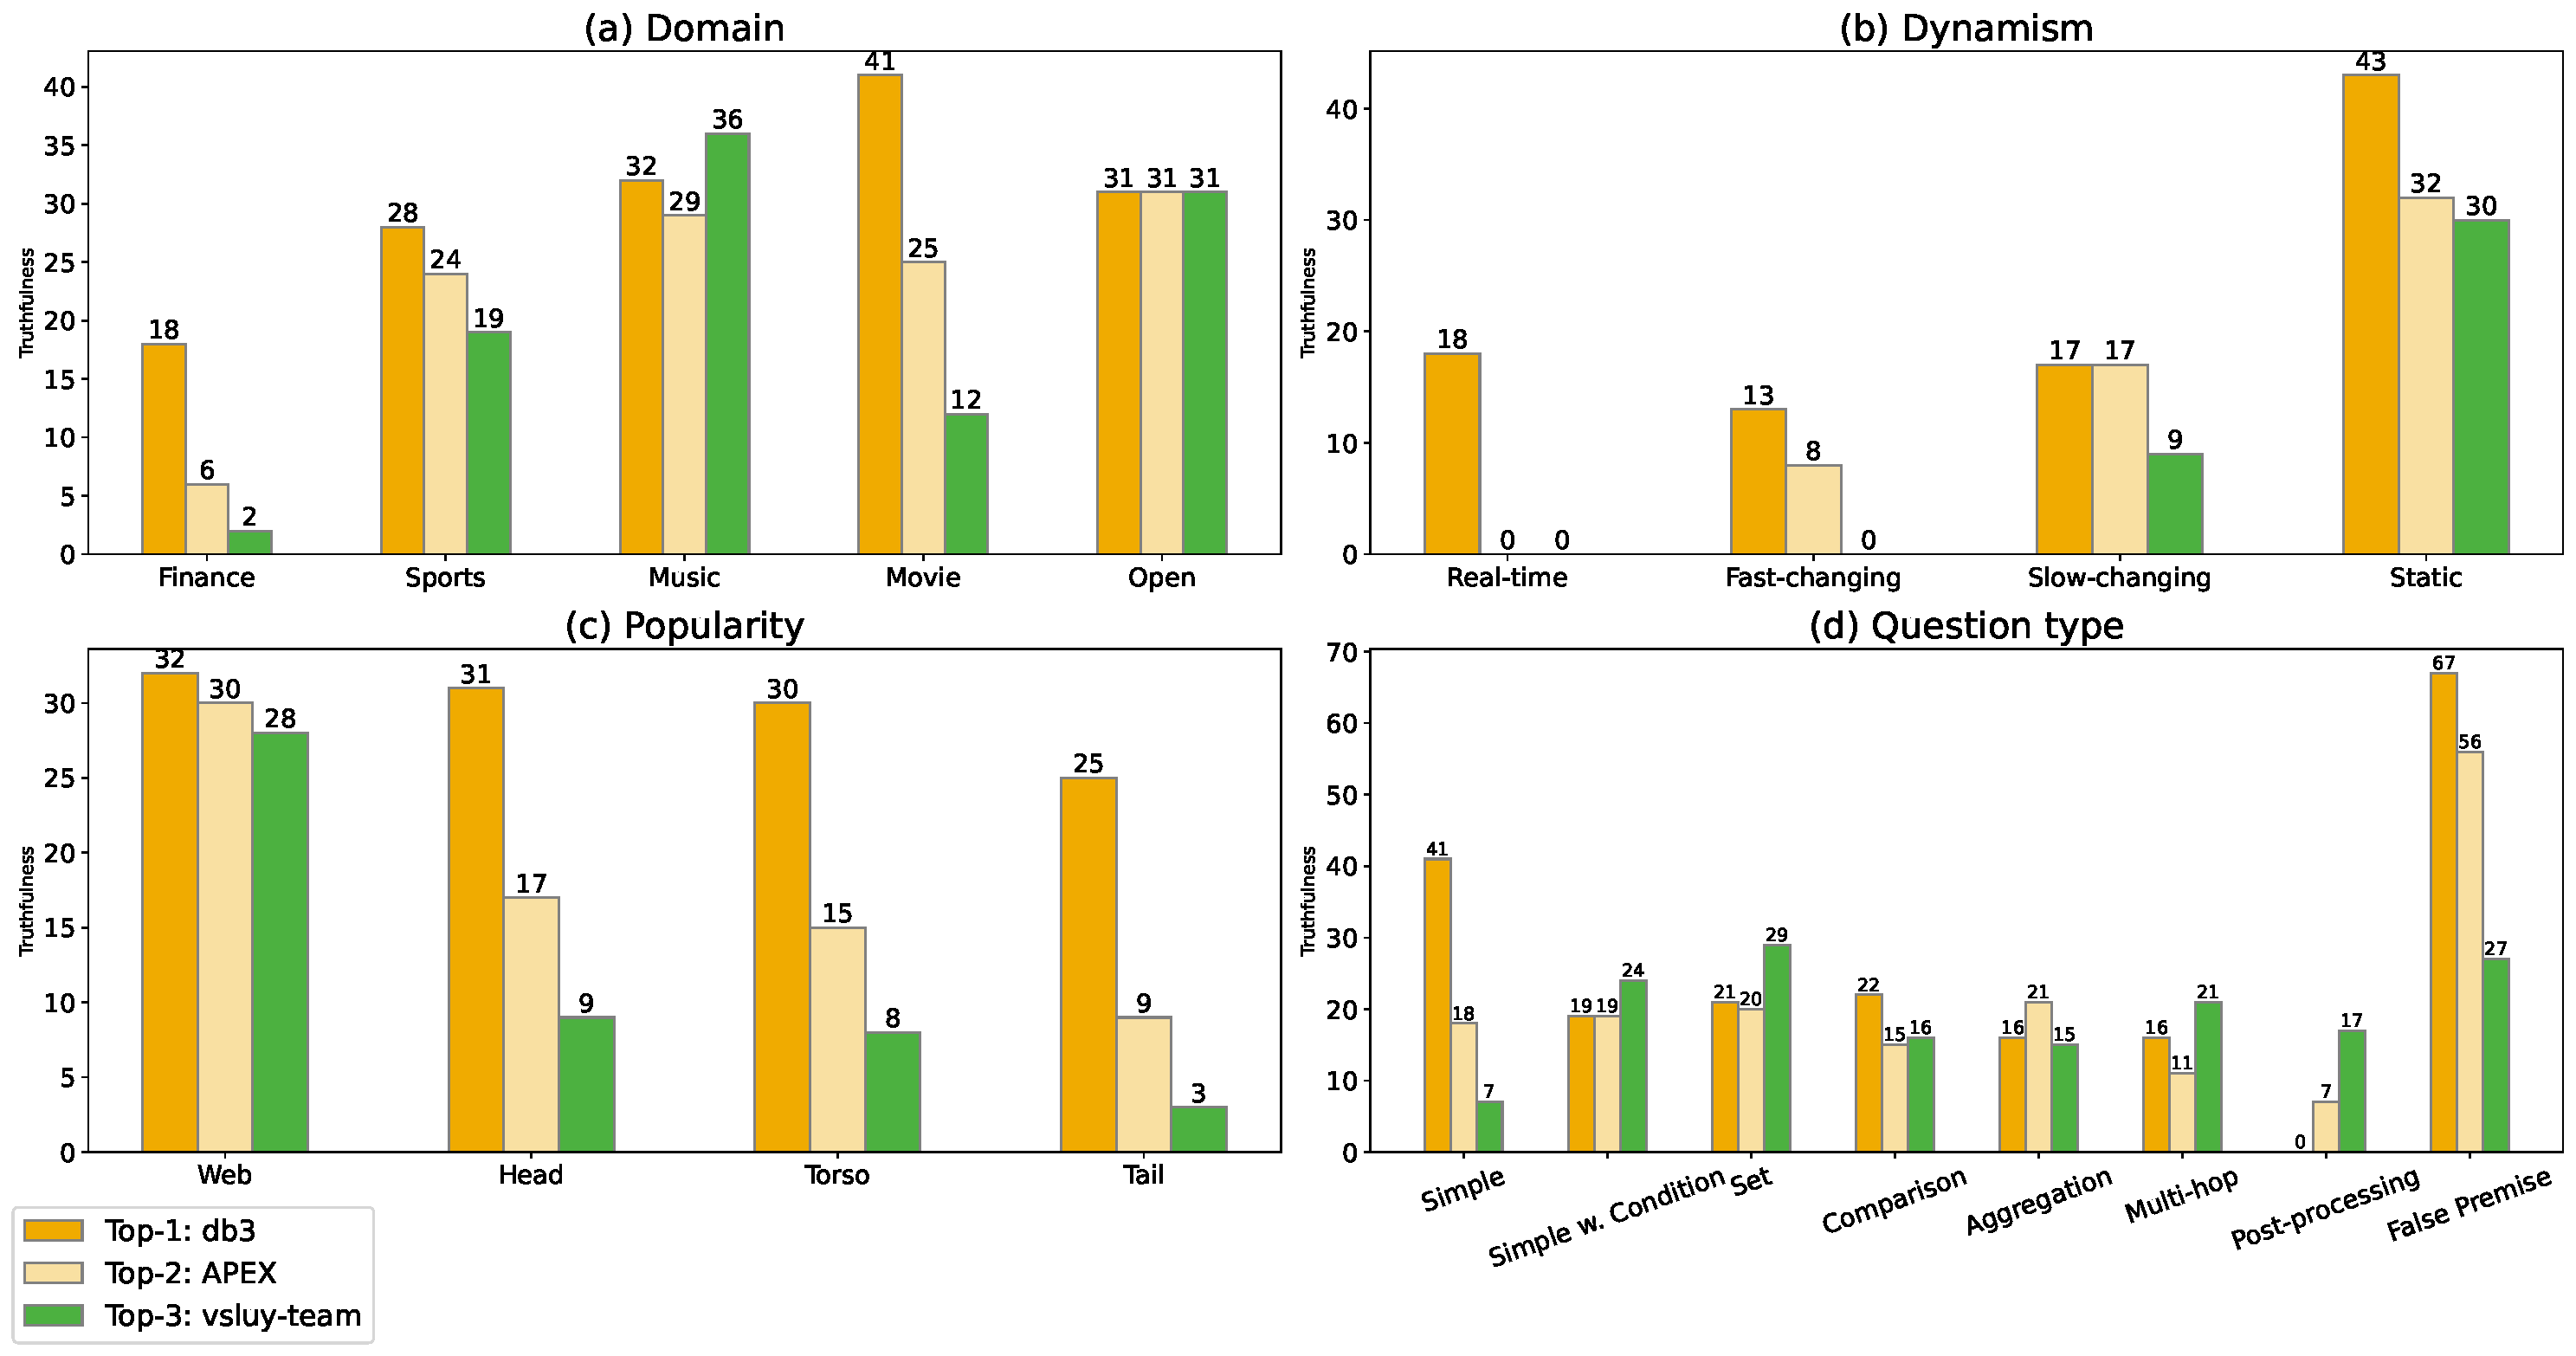
\includegraphics[width=16cm]{submissions/Xiao2024/figs/task_3_winner_slicing.pdf}
  \caption{Human-evaluated Truthfulness scores from Task 3 winners on the private test set across the four question categories. The truthfulness scores reflect different strategies taken by different winning teams. First-place winner for all three tasks Db3 \cite{db3}, as an example, put in significant efforts for improving the results on using the APIs, which gained them large margins in handling those KG-supported questions.}
  \label{fig:question category}
\end{figure}

\paragraph{Domain dimension} Since each domain has its own set of APIs, most winning solutions develop router to detect the topic domain of each question then use the results to select appropriate API calls and construct domain specific prompts accordingly. 

Among the domains, Finance questions prove to be the most challenging. This is mainly because many financial questions are real-time or fast-changing (e.g., "can you tell me the opening stock price of landp on the last Friday (question asked on 02/28/2024, 07:58:48 PT)?"), thus requiring finding results precisely corresponding to the reference time. To tackle date-time parsing, APEX~\cite{apex} leveraged regex rules and Python libraries (pytz and datetime) to parse absolute datetime objects. One other challenge is that Finance questions often require numeric reasoning. ElectricSheep \cite{electricsheep} delegates numeric calculations to an external Python interpreter, which reduces hallucination from LLM. 

\paragraph{Dynamism dimension} Overall, winning solutions perform better in static and slow-changing questions than fast-changing and real-time questions, mainly because of difficulties in temporal reasoning in both the retrieval step and the summarization step. Some teams even implemented solutions to blankly answer ``I don't know" for all dynamic questions to reduce hallucination penalties. One promising approach was team db3's~\cite{db3} ``regularized" APIs (see Section \ref{sec: kg}), which improved the APIs' expressiveness in handling temporal information.

Dynamic questions are an area where RAG should excel over vanilla LLM. The fact that teams struggle with dynamic questions suggests further opportunities in this area.

\paragraph{Popularity dimension} In this dimension, the performance is largely correlated with entity popularity as expected, due to sparsity of information for torso to tail questions.

\paragraph{Question Type dimension} In this dimension, comparison questions (e.g., ``who started performing earlier, Adele or Ed Sheeran?”), post-processing questions (e.g., ``How many days did Thurgood Marshall serve as a Supreme
Court justice?"),  and multi-hop questions (e.g., ``what school does Lebron James's youngest son attend?") are the most difficult types, mainly because they require retrieving information of multiple entities and nontrivial reasoning over the retrieved results. 

Team dRAGonRAnGers's \cite{dragonrangers} solution won first place for comparison questions in all three tasks. The authors hypothesized that their explicit chain-of-thought prompt contributed to the success by generating rationals for each entities involved in the comparison then synthesizing a final answer. Similarly, carefully engineered chain-of-thought prompts also improved reasoning for multi-hop and post-processing questions, as Team ElectricSheep \cite{electricsheep} and bumblebee7 \cite{bumblebee7} demonstrated.

